\section{Attempts to break the claims}
\label{sec:break}

Every claim of this paper was attacked numerically before its proof was written, following a search plan fixed in advance.
For each claim we report the families searched, planted adversaries (``dips'' of known depth placed in the space of states, which the search must find), and deliberately wrong versions of the claim, which the same search must break.
A search that finds the planted dips and breaks the wrong versions has shown that it can see a failure; a search that finds nothing without this check shows little.
All statements of this section are \numst; none of them is used in a proof.
Table~\ref{tab:break} summarizes them.

\begin{table*}
\caption{Attempts to break the claims. ``Margin'' is the smallest value found of the quantity in the second column (the claim needs the value in brackets). ``Power'' lists deliberately wrong versions and how many of them the same search broke. All entries are \numst.}
\label{tab:break}
\begin{ruledtabular}
\small
\begin{tabular}{p{0.14\textwidth}p{0.18\textwidth}p{0.16\textwidth}p{0.19\textwidth}p{0.19\textwidth}}
claim & quantity [needed] & margin & families & power\\ \hline
Theorem~\ref{thm:narrow} (lines) & $(F^2-1)\ell$ of the best option [$10$] & $17.5547$ ($\ell=55.26$) to $64.0750$ ($\ell=10^8$) & 13 families, 10 values of $\ell$, $4.8\times10^4$--$1.3\times10^5$ states each & 12 planted dips found; 8 wrong versions broken (a line dropped, (J) dropped, one option only)\\
the rule of Sec.~\ref{sec:narrow} & $(F^2-1)\ell$ of the rule [$10$] & $17.5565$ ($\ell=55.26$), no state below & 4 values of $\ell$, 7{,}200--7{,}503 states each & ---\\
Theorem~\ref{thm:res} (lines) & $\gamma^*$ [$0.6$] & $0.7377$ ($\ell=55.26$, $b=1$) & 6 values of $\ell$, about 23{,}500 points each & planted dip found; P1, P4z or (CM) dropped: broken; claim $\gamma^*\ge0.8$: broken\\
Theorem~\ref{thm:wide} (lines) & $(F^2-1)\ell$ of the rule [$10$] & $576.3$ ($\ell=960.8$, $B=8\ell+100$) & 13 families $+$ wide-focus families, $\ell$ up to $10^9$ & 7 planted dips found; cKz, P1 or (J) dropped, one option only: broken\\
Proposition~\ref{prop:BE} & $((a)+(a'))\sigma/\kappa(B)$ [$1$] & $3.56$ (197 states); $1.21$ (24 planted tight states) & true quantity, $\ell=6,8,10$ & $0.459\to0.6,0.75,1.0$: broken in 6, 14, 20 states; $(1-e)\to1$: 42; $\Psi\to1$: 27\\
Lemma~\ref{lem:R} & remainders [$\le2\times10^{-4}$] & $4.76\times10^{-9}$ & 10{,}245 points of $(\ell,\tau,B)$ & $\tau_0=2\ln\ell+10$: $\ge8.40$; $\nu\sim e^{-\tau/4}$: $\ge0.100$\\
Lemma~\ref{lem:P} & $N_\phi/(c_P(b+W))$ [$1$] & $1{,}482$ (117 states); $1{,}683$ (20 states, non-Gaussian $\Gamma$) & true quantity, $\ell=6,8$, $\tau$ from $0.06$ to $1800$ & $\theta\to\frac15$: broken in 2 states (8 with non-Gaussian $\Gamma$)\\
steps of Lemma~\ref{lem:P} & $\phi/\phi_r$; $\int_{I^c}q/(\theta\int_Iq)$ [$1$] & $2.46$; $39.6$ & 45 states $\times$ 11 values of $w$ & $\phi_r\times4$: broken in all 45; $\theta\to\frac15$: 3\\
\end{tabular}
\end{ruledtabular}
\end{table*}

\subsection{The lines (Theorems~\ref{thm:narrow}--\ref{thm:wide})}

\emph{What is searched.}
The claims of Propositions~\ref{prop:narrow}, \ref{prop:res} and~\ref{prop:wide} are statements about the sums of lines over the whole state space allowed by (H$'$): $\mu\in[e^{-3\ell},8\ell+80]$, $r\in[\sigma^3,\tfrac14]$, $\kappa\in[e^{-2.2\ell-50},e^{3\ell}]$, $B$ in its band, and $P$ up to the ceiling of (H$'$).
$F$ denotes the ratio of the lines' value to the target, and the claim $\Lambda\ge0$ with $\gamma=\Gamma_\ell$ is $(F^2-1)\ell\ge10$.

\emph{Results.}
For Theorem~\ref{thm:narrow} the smallest value is $17.5547$ at $\ell=55.26$ and grows slowly with $\ell$ (Fig.~\ref{fig:cases}b).
It sits in every case at the same corner: $\mu\approx\ell/4-\delta$, $r\approx\sigma^{1/2}$, $b\approx\sigma$, the brightness at its ceiling, and the option Tz-B1.
For Theorem~\ref{thm:res} the smallest $\gamma^*$ is $0.7377$, at $b=1$, $r=\tfrac14$ and the brightness at its ceiling, and no state of Case~II exists there.
For Theorem~\ref{thm:wide} the smallest value of the rule's branch is $576.3$ at $\ell=960.8$ and $B=8\ell+100$, far above $10$; the best option gives at least $2.16\times10^5$ in this band.
The rule's branch is smallest where the rule switches from Case~I to Case~II; this is set by the rule constant $c_1$, not by a hard state.

\emph{Power.}
Dropping any of the lines P1, P2z, hFz, P4z or cKz, dropping (J) from (H$'$), or keeping only Fz or only Tz-B2, breaks Theorem~\ref{thm:narrow} at $\ell=55.26$ and $955.8$.
Some versions are not broken: the option Tz-B1 alone suffices numerically, and removing the lower end of $b$ or either end of $a$ does not break the claim.
The proof uses those ends, but they are not numerically necessary.
At $\ell=955.8$ (not at $55.26$), the pairs $\lambda\approx1$ of (J) are needed.
The planted dips of depth $5$ at the corner, at narrow states and at low $\mu$, each with two widths and at $\ell=165.78$ and $10^5$, are all found.
The first version of the search missed four of them, because only the 40 globally lowest points were refined; the search was changed to refine the best point of every family.

\emph{The lines against the lemmas.}
That each line is a lower bound for the term of the lemma it comes from was audited in $64$ to $84$ decimal digits at $12$ values of $\ell$ from $55.26$ to $10^{12}$ ($1{,}500$ states each), with no violation; deliberately altered lines are caught.
The $30$ groups of formulas behind the lines were checked step by step at $37{,}886$ points, with no failure.

\subsection{The very wide focus (Theorem~\ref{thm:verywide})}

\emph{The true quantities.}
For Proposition~\ref{prop:BE} and Lemma~\ref{lem:P} we compare with the true $(a)+(a')$ and $N_\phi$ computed by direct two-dimensional quadrature, with the $v$-grid following the highest harmonic up to $200{,}001$ points.
Double precision reaches only $\sigma=e^{-\ell}$ with $\ell\le10$, where the regime $x\ge5\times10^{11}\sigma^2$ cannot hold.
These comparisons test the formulas at small $\ell$; they are evidence about the formulas, not about the theorems.
For Proposition~\ref{prop:BE} we impose $B\ge200/\tau$, i.e.\ $\beta\le0.05\tau$, as the small-$\ell$ analogue of $\beta\le10^{-6}\tau$.

\emph{Results.}
On $197$ states ($B\in[0.16,300]$, $\tau\in[40,1500]$, one to five harmonics, envelopes at the ends and in the middle of the class) the ratio $((a)+(a'))\sigma/\kappa(B)$ is at least $3.56$, and the collected inequality of the proof holds in all of them (Fig.~\ref{fig:true}).
\emph{A wrong expectation.}
We expected the version with $0.459$ replaced by $0.6$ to break where the ripple dominates.
It did not, because a wide envelope makes the term $eW\Phi$ that the proof drops large.
We then planted $24$ states where the bound should be tight (narrow envelope $L^2=c/B$, one strong high harmonic, $W/b$ of $3{,}000$ to $6{,}000$, $\ell=10$): the ratio is at least $1.21$, and the versions with $0.6$, $0.75$ and $1.0$ break in $6$, $14$ and $20$ of them.
The constant $0.459$ has about $20\%$ room where we can measure it.
For Lemma~\ref{lem:P} the bound has a large margin ($1{,}482$ and more); its steps (i) and (ii) were checked separately at fixed $w$.
The steps hold with margins $2.46$ and $39.6$; the minimum of $\phi/\phi_r$ is close to $\pi^2/4$, which is the gap between $1-\cos u\ge2u^2/\pi^2$ and $u^2/2$.
Measured directly, $N_\phi\cdot8B/(b+W)\ge1.000$ for $B\ge3$, so the true $N_\phi$ is close to $(b+W)/(8B)$ \numst.

\begin{figure}
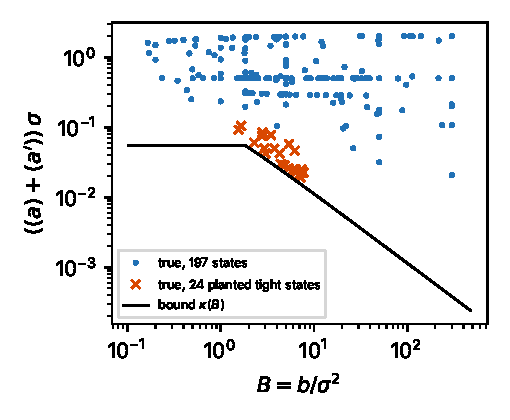
\includegraphics[width=\columnwidth]{figures/fig_true.pdf}
\caption{Proposition~\ref{prop:BE} against the true quantity, by direct quadrature at $\ell=6,8,10$ (material, outside the regime of the theorem). Dots: $((a)+(a'))\sigma$ for the 197 states with $\tau\ge40$ and $B\ge200/\tau$. Crosses: the 24 planted tight states. Line: the bound $\kappa(B)=\min(0.055,0.459/(4B+1))$. \numst}
\label{fig:true}
\end{figure}

\emph{Picture.}
The searches look in every corner of the space of states and find the hardest point of each claim, and in every case it lies above what the law asks.
The hardest states are always of the same kind: the ripple is as bright as positivity allows, and it sits where the focus is about to stop helping.
